\section{Experimentation} We train 90\% of our data using different combinations
of features and test them on the remaining 10\%. We take the features in the
following combinations -- only unigrams, unigrams + filtered bigrams and
trigrams, unigrams + negation, unigrams + filtered bigrams and trigrams +
negation. We then train classifiers using different classification
algorithms -- Naive Bayes Classifier and Maximum Entropy Classifier.

The task of classification of a tweet can be done in two steps -- first,
classifying ``neutral'' (or ``subjective'') vs. ``objective'' tweets and second,
classifying objective tweets into ``positive'' vs. ``negative'' tweets. We also
trained 2 step classifiers. The accuracies for each of these configuration are 
shown in \figref{fig:nbme_acc}, we discuss these in detail below.

\begin{figure}[h!]
\centering
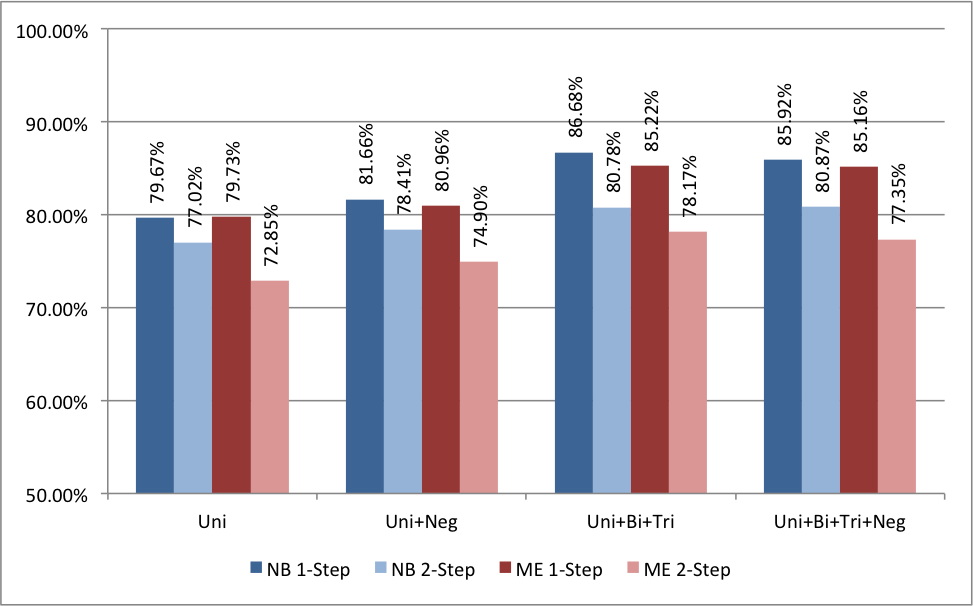
\includegraphics[width=\textwidth]{img/NBME_Accuracy.png}
\caption{Accuracy for Naive Bayes Classifier}
\label{fig:nbme_acc}
\end{figure}


\subsection{Naive Bayes} Naive Bayes classifier is the simplest and the fastest
classifier. Many researchers \cite{GBH}, \cite{PP} claim to have gotten best
results using this classifier.

For a given tweet, if we need to find the label for it, we find the
probabilities of all the labels, given that feature and then select the label
with maximum probability.

\begin{equation}
label_{NB} := argmax_{label} P(label|features)
\end{equation}

In order to find the probability for a label, this algorithm first uses the
Bayes rule to express P(label|features) in terms of P(label) and
P(features|label) as,

\begin{equation}
P(label|features)
	= \frac	{P(label) * P(features|label)}
			{P(features)}
\end{equation}

%Bayes rule to express $P(label|features)$
%P(label│features)=  (P(label)*P(features|label))/(P(features))

Making the `naive' assumption that all the features are independent,

\begin{equation}
P(label|features)
	= \frac	{P(label) * P(f_1|label) * ... * P(f_n|label)}
			{P(features)}
\end{equation}

%Naive assumption of independent features
%P(label│features)=  (P(label)*P(f1│label)…*P(fn|label))/(P(features))

Rather than computing P(featues) explicitly, we can just calculate the
denominator for each label, and normalize them so they sum to one:

\begin{equation}
P(label|features)
	= \frac	{P(label) * P(f_1|label) * ... * P(f_n|label)}
			{\sum_l( P(l) * P(f_1|l) * ... * P(f_n|l) )}
\end{equation}

%Normalise the denominator
%P(label│features)=  (P(label)*P(f1│label)…*P(fn|label))/(∑_l▒〖(P(l)*P(f1│l)*…*P(fn|l))〗)

The results from training the Naive Bayes classifier are shown below in
\figref{fig:nbme_acc}. The accuracy of Unigrams is the lowest at 79.67\%. The
accuracy increases if we also use Negation detection (81.66\%) or higher order
n-grams (86.68\%). We see that if we use both Negation detection and higher
order n-grams, the accuracy is marginally less than just using higher order
n-grams (85.92\%). We can also note that accuracies for double step classifier
are lesser than those for corresponding single step.

%\begin{figure}[h!]
%\centering
%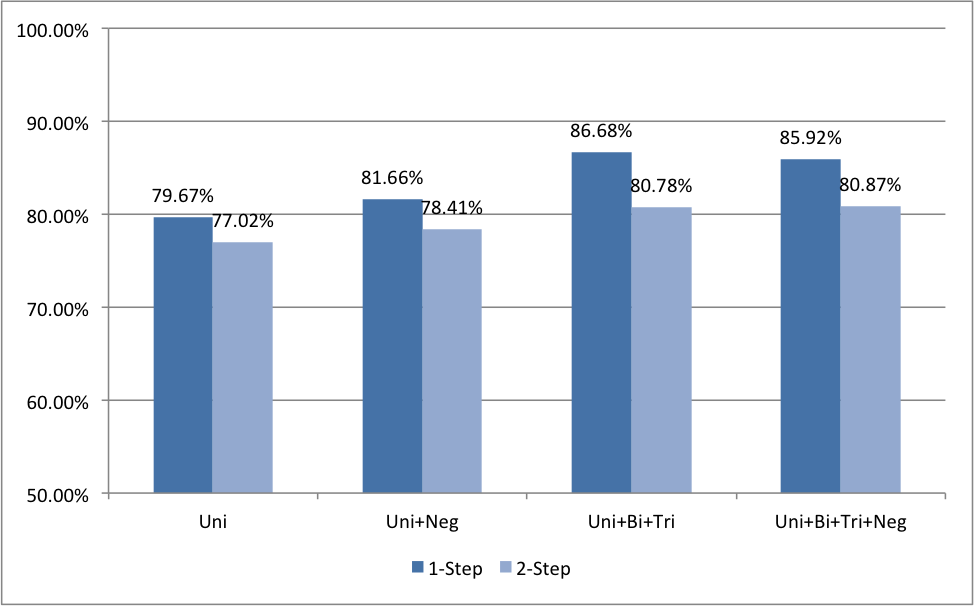
\includegraphics[width=\textwidth]{img/NB_Accuracy.png}
%\caption{Accuracy for Naive Bayes Classifier}
%\label{fig:nb_acc}
%\end{figure}
%Figure 9: Accuracy for Naive Bayes Classifier

We have also shown Precision versus Recall values for Naive Bayes classifier
corresponding to different classes – Negative, Neutral and Positive in
\figref{fig:nb_pr}. The solid markers show the P-R values for single step
classifier and hollow markers show the affect of using double step classifier.
Different points are for different feature sets. We can see that both precision
as well as recall values are higher for single step than that for double step.

\begin{figure}[h!]
\centering
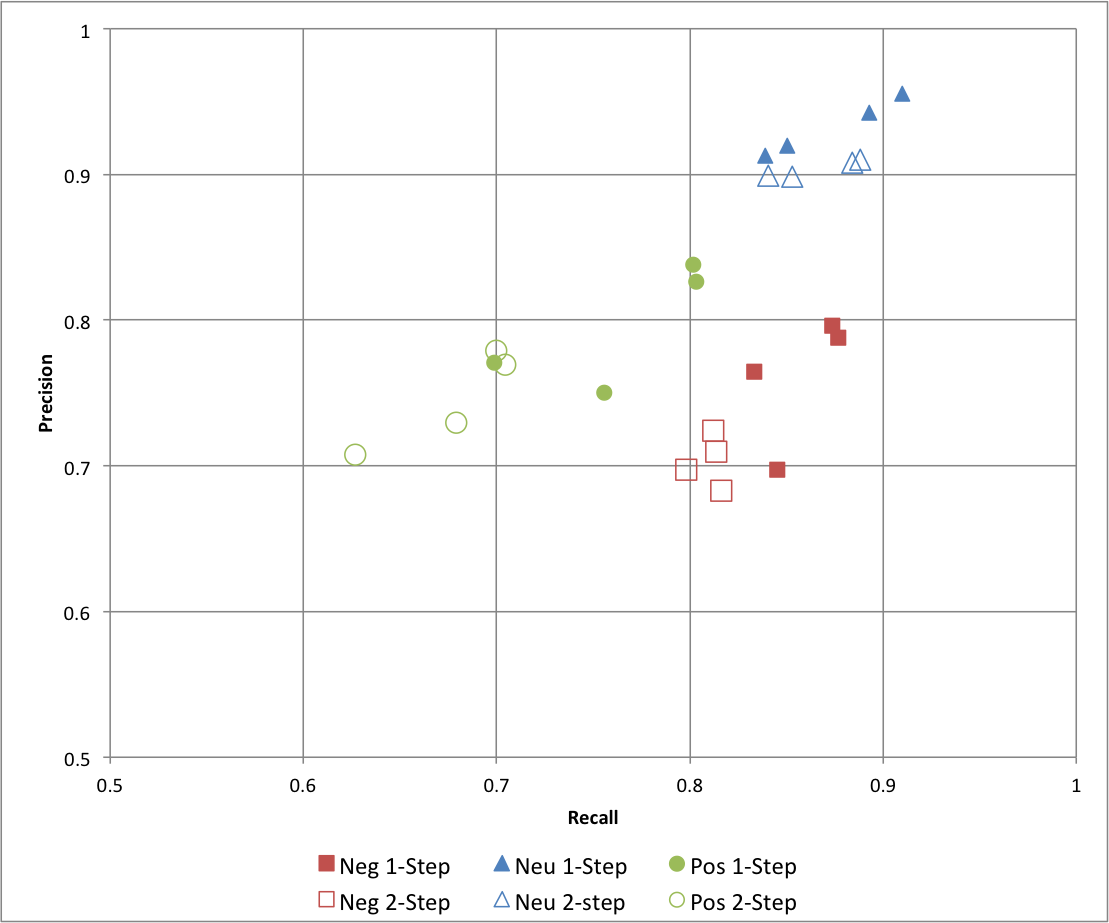
\includegraphics[width=\textwidth]{img/NB_PvsR.png}
\caption{Precision vs. Recall for Naive Bayes Classifier}
\label{fig:nb_pr}
\end{figure}
%Figure 10: Precision vs. Recall for Naive Bayes Classifier


\subsection{Maximum Entropy Classifier}

This classifier works by finding a probability distribution that maximizes the
likelihood of testable data. This probability function is parameterized by
weight vector. The optimal value of which can be found out using the method of
Lagrange multipliers.

\begin{equation}
P(label|features)
	= \frac	{\sum_i  w_i f_i(label)}
			{\sum_{l \in labels} \sum_i  w_i f_i(l) }
\end{equation}

The results from training the Naive Bayes classifier are shown below in
\figref{fig:nbme_acc}. Accuracies follow a similar trend as compared to Naive
Bayes classifier. Unigram is the lowest at 79.73\% and we see an increase for
negation detection at 80.96\%. The maximum is achieved with unigrams, bigrams
and trigrams at 85.22\% closely followed by n-grams and negation at 85.16\%. Once
again, the accuracies for double step classifiers are considerably lower.

%\begin{figure}[h!]
%\centering
%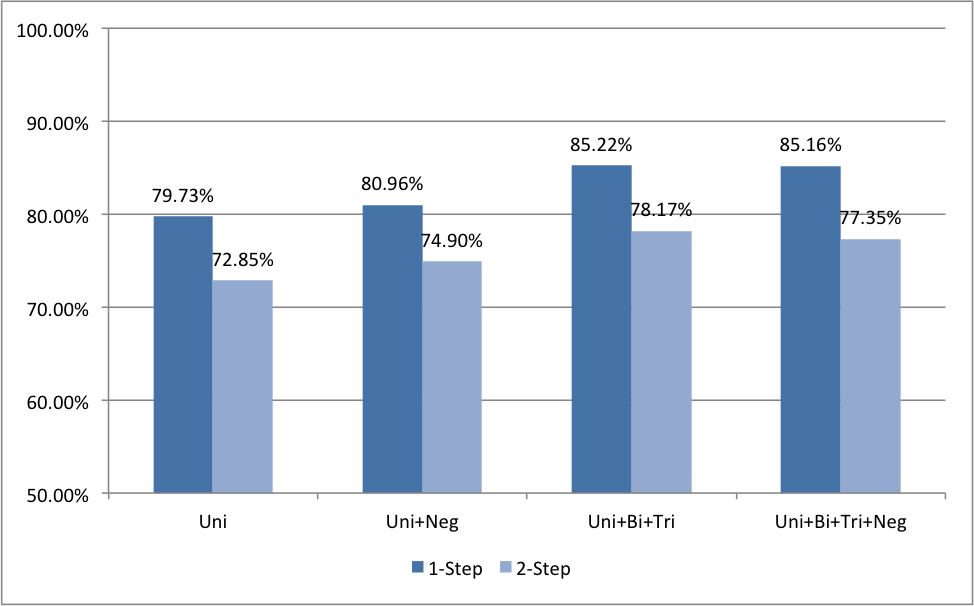
\includegraphics[width=\textwidth]{img/ME_Accuracy.png}
%\caption{Accuracy for Maximum Entropy Classifier}
%\label{fig:me_acc}
%\end{figure}
%Figure 11: Accuracy for Maximum Entropy Classifier

Precision versus Recall map is also shown for maximum entropy classifier in
\figref{fig:me_pr}.  Here we see that precision of ``neutral'' class increase by
using a double step classifier, but with a considerable decrease in its recall
and slight fall in precision of ``negative'' and ``positive'' classes.

\begin{figure}[h!]
\centering
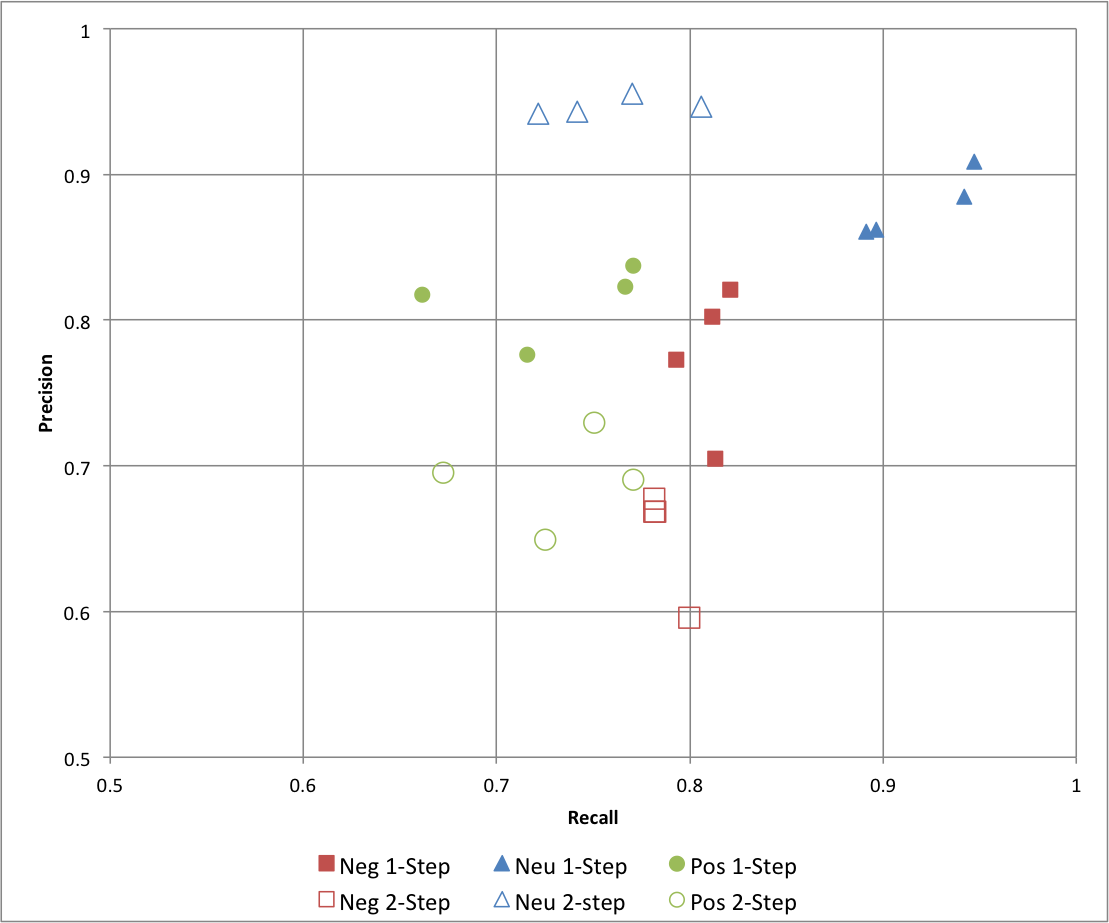
\includegraphics[width=\textwidth]{img/ME_PvsR.png}
\caption{Precision vs. Recall for Maximum Entropy Classifier}
\label{fig:me_pr}
\end{figure}
%Figure 12: Precision vs. Recall for Maximum Entropy Classifier